This section describes the data model used in Obvious and the way to
create data structures. It also exposes the util package for the data
model.  The data model used in Obvious has been largely specified
during the workshop: a consensus has been found among all
participants.

\begin{figure}[!h]
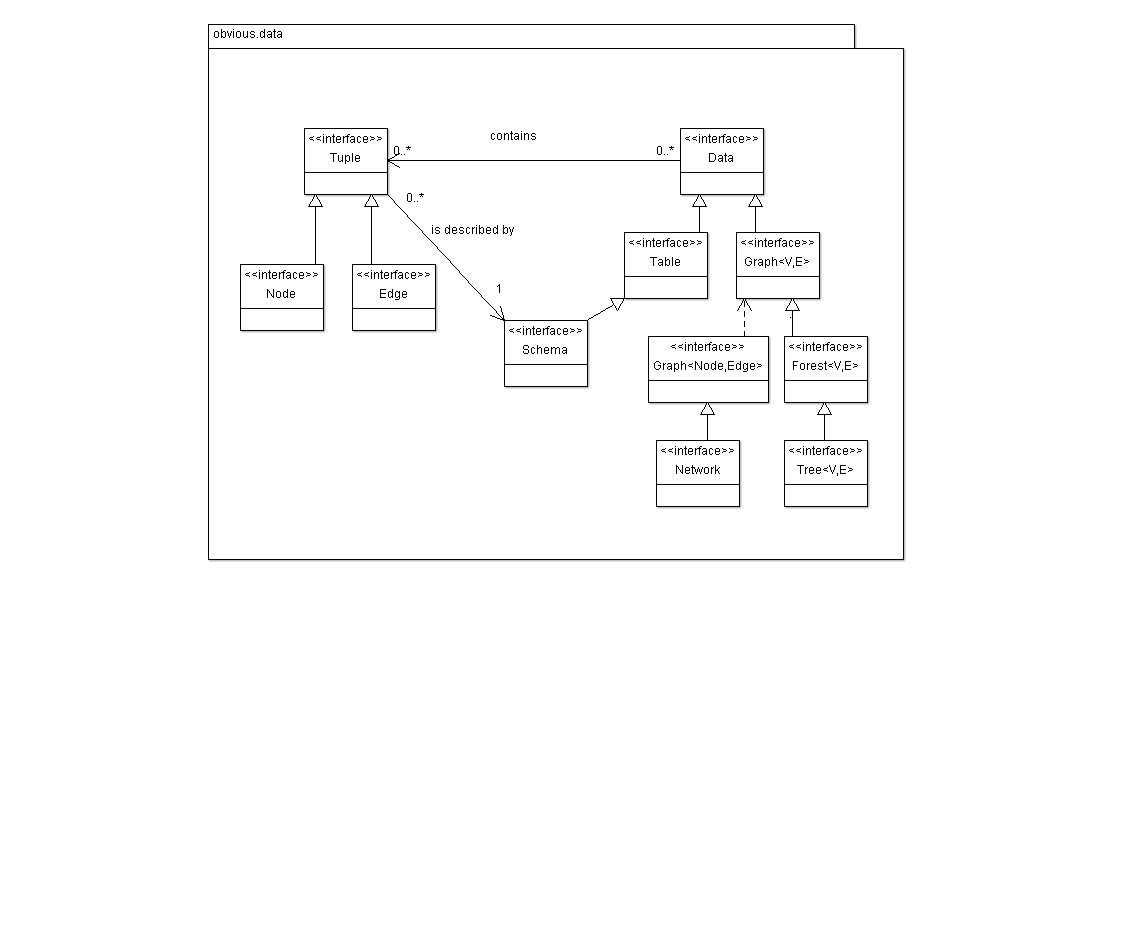
\includegraphics[width=\columnwidth]{figures/obviousdataclass}
\caption{Class diagram of the data model}
\label{fig:datamodel}
\end{figure}

The initial data model proposed for Obvious derived from the proxy tuple
design pattern exposed in \cite{DesignPatternsIV}. However, originally, this model
contained table, graph and tree (an extension of graph) classes. The initial proposal
used the relational graph pattern described in \cite{DesignPatternsIV}. 
While this pattern facilitates extendability, graphs cannot be manipulated in an
object-oriented manner and as many developers are used to manipulation of
 \emph{object oriented graphs}, the relational graph pattern was not considered
 satisfactory.  We therefore offered the use of the proxy tuple pattern, a
design pattern combining benefits of the relational graph pattern and
of object oriented graphs.

In addition, a major difference exists between our patterns and those
introduced in \cite{DesignPatternsIV}. Our patterns used schema to describe
the columns of a table (type, name and default value) instead of a column object,
that does not exist in Obvious. Schemas have been introduced, since it
is efficient to gather all \emph{meta-data} for the columns of a
table in one unique structure, allowing table and network instantiations
with a factory.

Thus, the data model used in every implementation [described in the
  corresponding section] is built around tuples: abstractly tables are
composed of tuples and graphs are described as networks i.e. a
combination of two tables one made of nodes and the other of edges
(both classes derived from tuples).

Also, this model is completed by factories, that allows data structure
instantiations. Logically, they used the well known factory
pattern. With those factories, it is possible to instantiate tables
and networks from a schema or from an existing object from a targeted
Obvious implementation (e.g. a Prefuse table or a JUNG graph...). This also
provides the possibility to use parameters to provide more arguments
used in targeted toolkits. For example, in the Prefuse implementation
of Obvious, parameters are used to specify the source and target node columns
for a graph in an edge table.

Finally, we have defined an utility package obviousx, named in the
same way as javax. This package provides different kinds of utility
classes for the Obvious data model. First, we have defined in
obviousx, reader and writer interfaces allowing the creation of gateways
between the Obvious data model and common data formats such as CSV and
GraphML. It is useful since it gives software developers a standard
way to import and export data in Obvious whatever the underlying
implementation of the data model is. In addition, for data providers,
it simplifies their work because they only have to develop one reader
and one writer to be compatible with a large number of toolkits. With
the same logic, obviousx furnishes a Java TableModel compatible with
the Obvious one: it allows quick creation of a JTable from an Obvious
table. Finally, obviousx also provides wrappers to \emph{transform}
obvious data structures into common existing data structures (Prefuse,
Ivtk, Jung, more to develop) in order to avoid copying of data when using more than
one data model.
 
